\documentclass[border=4pt]{standalone}
\usepackage{amsmath,amssymb,amsfonts}
\usepackage{xcolor,colortbl,array,booktabs,multirow}
\usepackage{tikz}
\usepackage{pgfplots}
\pgfplotsset{compat=1.16}
\usetikzlibrary{arrows, automata, backgrounds, calendar, chains, decorations,
    matrix, mindmap, patterns, petri, positioning, shadows, shapes.geometric,
    trees, shapes, decorations.pathreplacing, calc, tikzmark, arrows.meta,
    intersections, fit, graphs, quotes, angles, decorations.markings}
\newcommand{\st}{\text{ s.t. }}
\newcommand{\x}{\mathbf{x}}
\renewcommand{\b}{\mathbf{b}}
\renewcommand{\c}{\mathbf{c}}
\newcommand{\A}{\mathbf{A}}
\newcommand{\y}{\mathbf{y}}
\newcommand{\z}{\mathbf{z}}
\newcommand{\R}{\mathbb{R}}
\newcommand{\RR}{\mathbb{R}}
\newcommand{\Z}{\mathbb{Z}}
\newcommand{\ZZ}{\mathbb{Z}}
\newcommand{\npcomplete}{NP-complete}
\providecommand{\true}{\text{TRUE}}
\providecommand{\false}{\text{FALSE}}
\tikzset{vertex/.style={circle,fill=black!25,minimum size=20pt,inner sep=0pt},
    edge/.style={draw,thick,-},weight/.style={font=\small},
    selected vertex/.style={vertex, fill=red!24},
    selected edge/.style={draw,line width=2pt,-,red!50},
    ignored edge/.style={draw,line width=2pt,-,black!20}}
\newcommand{\vect}{\vec}
\providecommand{\ds}{\displaystyle}
\providecommand{\longvect}{\overrightarrow}
\usepackage[normalem]{ulem}
\definecolor{ocre}{RGB}{243,102,25}
\providecommand{\leftB}{\left[}
\providecommand{\rightB}{\right]}
\tikzset{directed/.style={postaction={decorate,decoration={markings,mark=at position .65 with {\arrow{>}}}}},
    directed1/.style={postaction={decorate,decoration={markings,mark=at position .65 with {\arrow{>}}}}}}
\begin{document}
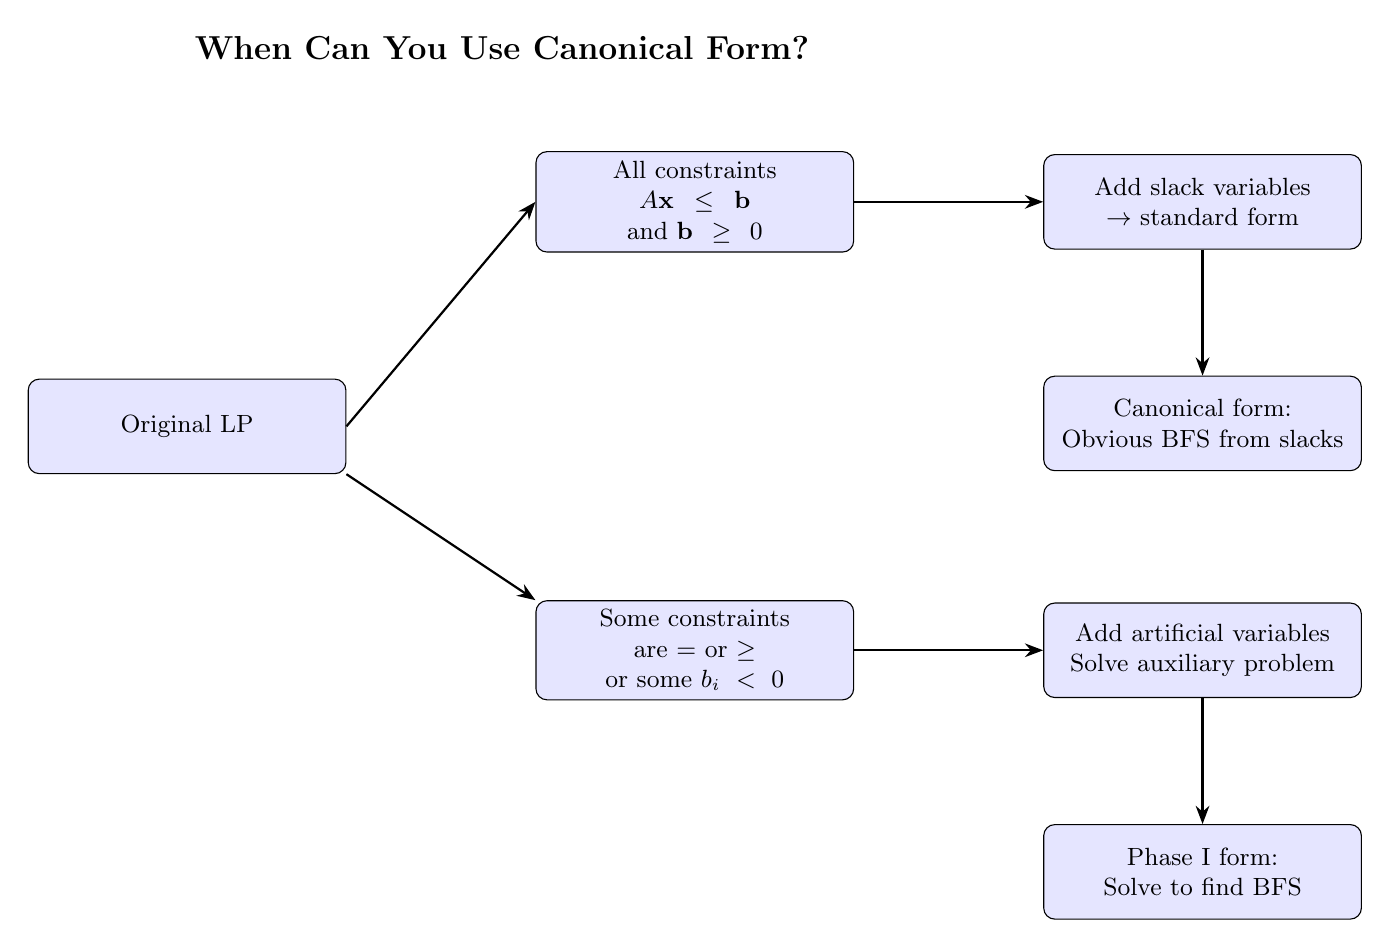
\begin{tikzpicture}[
  node distance=1.6cm and 2.4cm,
  every node/.style={font=\small},
  box/.style={draw, rounded corners, fill=blue!10, text width=3.8cm, align=center, minimum height=1.2cm},
  arrow/.style={-{Stealth}, thick}
]

% Nodes
\node[box] (start) {Original LP};
\node[box, above right=of start] (case1) {All constraints\\ $A\mathbf{x} \leq \mathbf{b}$\\ and $\mathbf{b} \geq 0$};
\node[box, right=of case1] (stdform) {Add slack variables\\ $\rightarrow$ standard form};
\node[box, below=of stdform] (canonform) {Canonical form:\\ Obvious BFS from slacks};

\node[box, below right=of start] (case2) {Some constraints\\ are $=$ or $\geq$\\ or some $b_i < 0$};
\node[box, right=of case2] (phase1) {Add artificial variables\\ Solve auxiliary problem};
\node[box, below=of phase1] (phase1form) {Phase I form:\\ Solve to find BFS};

% Arrows
\draw[arrow] (start.east) -- (case1.west);
\draw[arrow] (case1.east) -- (stdform.west);
\draw[arrow] (stdform.south) -- (canonform.north);

\draw[arrow] (start.south east) -- (case2.north west);
\draw[arrow] (case2.east) -- (phase1.west);
\draw[arrow] (phase1.south) -- (phase1form.north);

% Title
\node[align=center, font=\bfseries\large] at (4,4.8) {When Can You Use Canonical Form?};
\end{tikzpicture}
\end{document}
